\subsection{Quantitative and Qualitative Results}
\label{sec:results}

% Table 1 — paste full numbers from the manuscript; do not invent values
% Table 1 — data from latex/MipNeRF360数据集/formatting-instructions-latex.tex (unchanged numbers)
\begin{table}[ht!]
\centering
\caption{\label{tab:mip360} Performance comparisons of sparse-view synthesis on Mip-NeRF 360 (4/6/9 views). LPIPS$^{*}$ denotes LPIPS $\times 10^{2}$.}
\setlength{\tabcolsep}{2.8mm}
\renewcommand{\arraystretch}{1.08}
\adjustbox{width=1\linewidth}{%
\begin{tabular}{c l | ccc | ccc | ccc}
\toprule
\multirow{2}{*}{}
  & \multirow{2}{*}{Methods}
  & \multicolumn{3}{c|}{Mip-NeRF 360 (4-view)}
  & \multicolumn{3}{c|}{Mip-NeRF 360 (6-view)}
  & \multicolumn{3}{c}{Mip-NeRF 360 (9-view)} \\
&
  & LPIPS$^{*}$$\downarrow$ & PSNR$\uparrow$ & SSIM$\uparrow$
  & LPIPS$^{*}$$\downarrow$ & PSNR$\uparrow$ & SSIM$\uparrow$
  & LPIPS$^{*}$$\downarrow$ & PSNR$\uparrow$ & SSIM$\uparrow$ \\
\midrule
\sidelabel{2}{NeRF-based}
  & RegNeRF
      & 19.88 & 12.59 & 0.841
      & 20.72 & 13.41 & 0.847
      & 19.70 & 13.68 & 0.852 \\
  & SparseNeRF
      & 17.76 & 12.83 & 0.845
      & 19.74 & 13.42 & 0.861
      & 21.56 & 14.36 & 0.873 \\
\addlinespace[4pt]
\sidelabel{5}{3DGS-based}
  & 3DGS
      &10.80 & 20.31 & 0.899
      &8.38 & 22.12 & 0.913
      &6.42 & 24.29 & 0.930 \\
  & CoR-GS
      &11.76 & 20.45 & 0.856
      &9.28 & 22.57 & 0.901
      &7.04 & 24.73 & 0.926 \\
  & DropGaussian
      &11.57 & 21.76 & 0.837
      &8.61 & 22.98 & 0.895
      &8.02 & 24.10 & 0.915 \\
  & D$^2$GS
      &\cellcolor{color_blue}2.58 &\cellcolor{blue!8}22.35 &\cellcolor{blue!8}0.923
      &\cellcolor{color_blue}2.34 &\cellcolor{blue!8}24.74 &\cellcolor{blue!8}0.937
      &\cellcolor{color_blue}2.11 &\cellcolor{blue!8}27.13 &\cellcolor{blue!8}0.941 \\
  & SynGS (Ours)
      &\cellcolor{blue!8}3.89 &\cellcolor{color_blue}25.91 &\cellcolor{color_blue}0.948
      &\cellcolor{blue!8}3.43 &\cellcolor{color_blue}27.93 &\cellcolor{color_blue}0.953
      &\cellcolor{blue!8}3.02 &\cellcolor{color_blue}29.21 &\cellcolor{color_blue}0.961 \\
\bottomrule
\end{tabular}%
}
\end{table}


\textbf{Mip-NeRF 360.}
Table~\ref{tab:mip360} reports the results on Mip-NeRF 360 under the 4-, 6-, and 9-view settings. SynGS achieves the highest PSNR and SSIM in all three settings, with the largest PSNR advantage appearing in the 4-view case, where it reaches 25.91~dB, 3.56~dB above D$^2$GS~\cite{Song26_D2GS}. The advantage remains clear as the number of input views increases. For LPIPS, however, D$^2$GS obtains lower values across the three settings.

% Table 2 — caption uses ``LLFF 360'' (locked)
% Table 2 — LLFF 360 (locked dataset name). Paste manuscript numbers; do not invent.
% LPIPS* = LPIPS $\times 10^{2}$ throughout this paper.
\begin{table}[t]
\caption{Performance comparisons of sparse-view synthesis on the LLFF 360 dataset (4/6/9 views). LPIPS$^{*}$ denotes LPIPS $\times 10^{2}$.}
\label{tab:llff}
\begin{center}
\begin{tabular}{|l|ccc|ccc|ccc|}
\hline
\rule[-1ex]{0pt}{3.5ex}
 & \multicolumn{3}{c|}{4 views} & \multicolumn{3}{c|}{6 views} & \multicolumn{3}{c|}{9 views} \\
\cline{2-10}
\rule[-1ex]{0pt}{3.5ex}
Method & LPIPS$^{*}$$\downarrow$ & PSNR$\uparrow$ & SSIM$\uparrow$ & LPIPS$^{*}$$\downarrow$ & PSNR$\uparrow$ & SSIM$\uparrow$ & LPIPS$^{*}$$\downarrow$ & PSNR$\uparrow$ & SSIM$\uparrow$ \\
\hline
\rule[-1ex]{0pt}{3.5ex}
% TODO: paste rows from manuscript Table 2 (baselines may differ from Table 1)
\multicolumn{10}{|l|}{\textit{TODO: fill from manuscript Table 2}} \\
\hline
\end{tabular}
\end{center}
\end{table}


\textbf{LLFF 360.}
The LLFF 360 results in Table~\ref{tab:llff} show a similar trend under highly sparse inputs. With four views, SynGS achieves the best PSNR, SSIM, and LPIPS among the compared methods, while under six views it obtains the highest PSNR and SSIM with LPIPS close to the best result. At nine views, the differences become smaller: D$^2$GS~\cite{Song26_D2GS} gives slightly higher PSNR and lower LPIPS, while CoR-GS~\cite{Zhang24_CoRGS} achieves slightly higher SSIM. The clearest advantage appears in the 4- and 6-view settings.

\textbf{Qualitative Results.}
Figure~\ref{fig:qualitative} shows the qualitative comparison under the 4-view setting on Mip-NeRF 360. Compared with the baseline methods, SynGS produces fewer floating artifacts and more complete object boundaries, while preserving finer structures in regions where several competing methods exhibit broken contours or missing details.

\begin{figure*}[t]
\centering
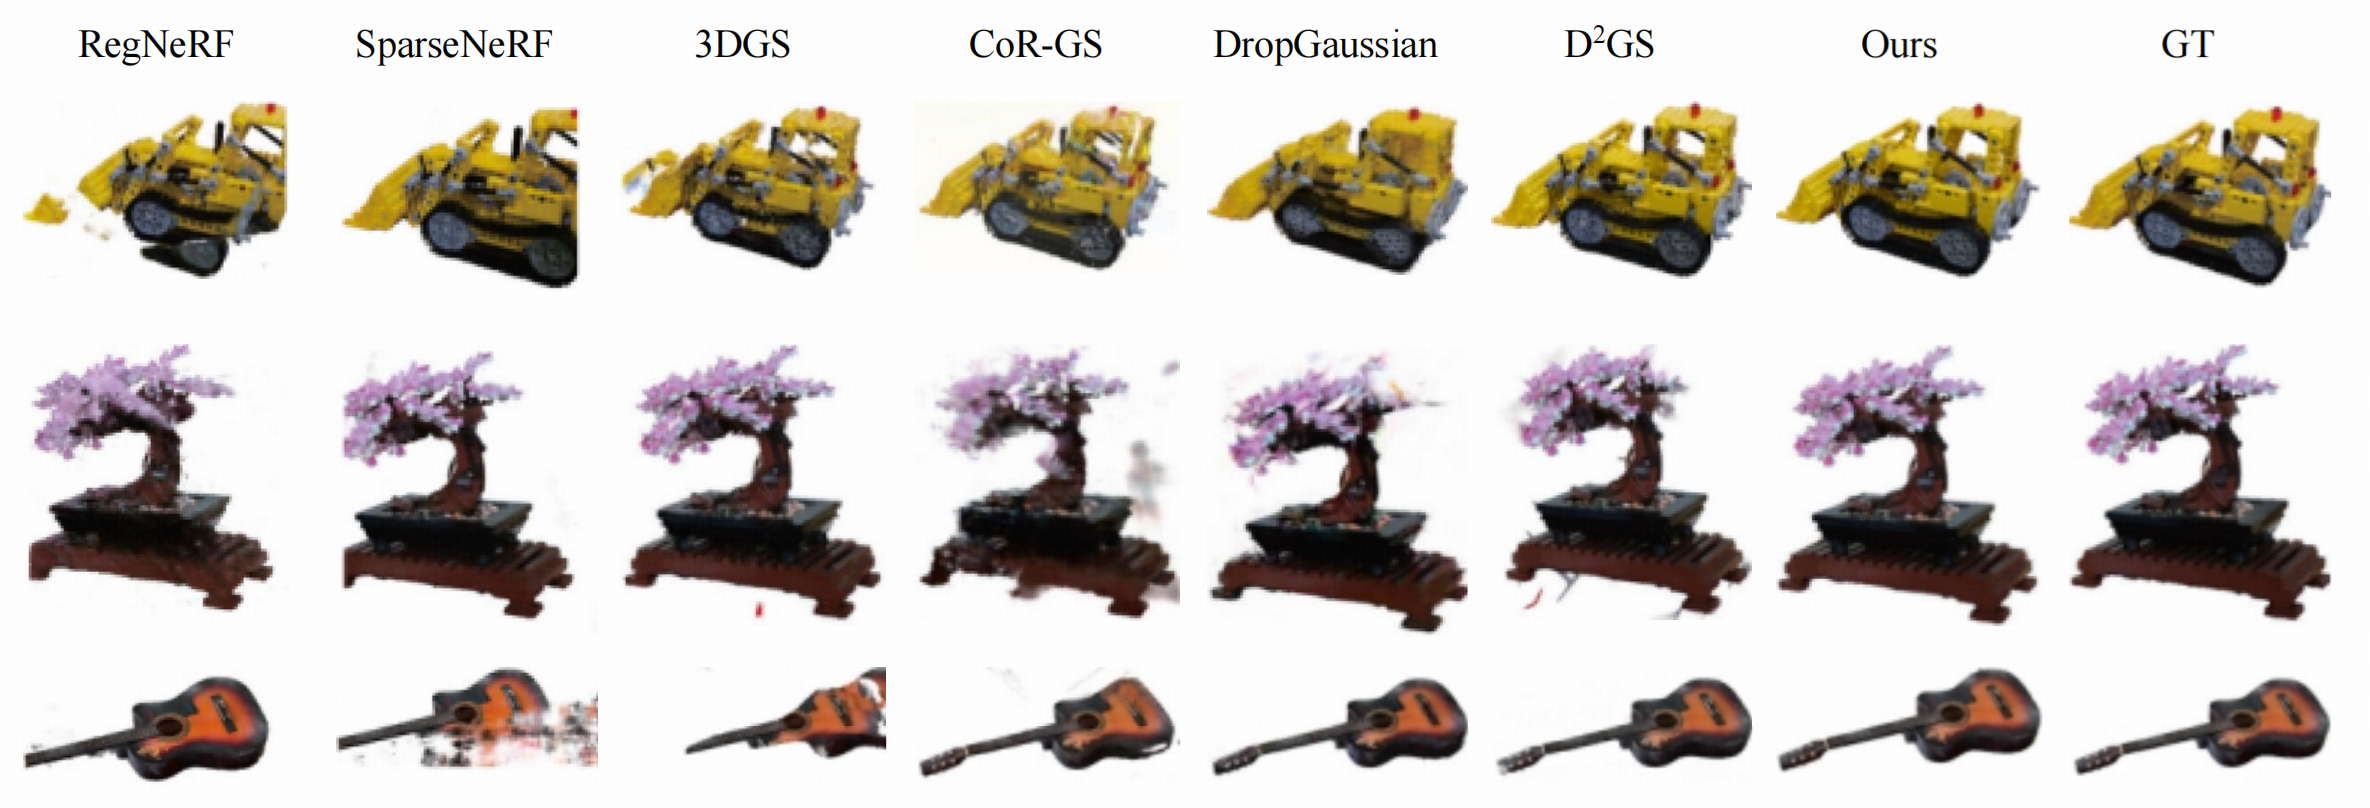
\includegraphics[width=\textwidth]{figures/qualitative.png}
\caption{Qualitative comparison under the 4-view sparse-input setting on Mip-NeRF 360. SynGS produces fewer floating artifacts and more complete structural boundaries than the compared methods.}
\label{fig:qualitative}
\end{figure*}
